\documentclass[tikz,border=8pt]{standalone}
\usepackage{tikz}
\usepackage{amsmath, amssymb}

\begin{document}

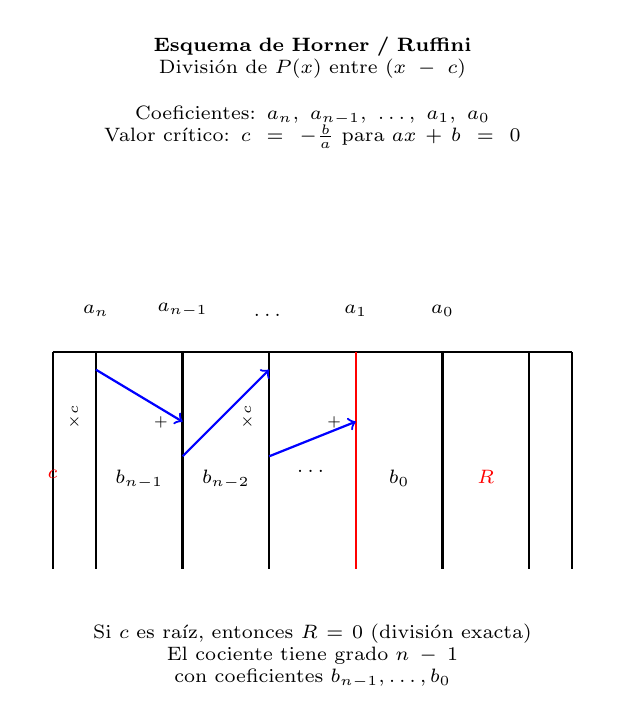
\begin{tikzpicture}[scale=1.1]

  % Esquema de Horner/Ruffini
  \node[align=center, text width=7cm, font=\scriptsize] at (0, 3) {
    \textbf{Esquema de Horner / Ruffini}\\
    División de $P(x)$ entre $(x - c)$\\
    \vspace{0.3cm}
    Coeficientes: $a_n,\ a_{n-1},\ \dots,\ a_1,\ a_0$\\
    Valor crítico: $c = -\frac{b}{a}$ para $ax+b=0$\\
  };

  % Tabla de Horner
  \draw[thick] (-3, 0) -- (3, 0);
  \draw[thick] (-3, 0) -- (-3, -2.5);
  \draw[thick] (3, 0) -- (3, -2.5);

  % Columnas
  \foreach \x in {-2.5,-1.5,-0.5,0.5,1.5,2.5} {
    \draw[thick] (\x, 0) -- (\x, -2.5);
  }

  % Líneas divisoria
  \draw[thick, red] (0.5, 0) -- (0.5, -2.5);

  % Etiquetas superiores (coeficientes del dividendo)
  \node[above, font=\scriptsize] at (-2.5, 0.3) {$a_n$};
  \node[above, font=\scriptsize] at (-1.5, 0.3) {$a_{n-1}$};
  \node[above, font=\scriptsize] at (-0.5, 0.3) {$\dots$};
  \node[above, font=\scriptsize] at (0.5, 0.3) {$a_1$};
  \node[above, font=\scriptsize] at (1.5, 0.3) {$a_0$};

  % Valor crítico c
  \node[below, font=\scriptsize, red] at (-3, -1.25) {$c$};

  % Resultados (cociente y residuo)
  \node[below, font=\scriptsize] at (-2, -1.25) {$b_{n-1}$};
  \node[below, font=\scriptsize] at (-1, -1.25) {$b_{n-2}$};
  \node[below, font=\scriptsize] at (0, -1.25) {$\dots$};
  \node[below, font=\scriptsize] at (1, -1.25) {$b_0$};
  \node[below, font=\scriptsize, red] at (2, -1.25) {$R$};

  % Operaciones
  \node[right, font=\tiny, rotate=90] at (-2.75, -1) {$\times c$};
  \node[right, font=\tiny, rotate=90] at (-1.75, -1) {$+$};
  \node[right, font=\tiny, rotate=90] at (-0.75, -1) {$\times c$};
  \node[right, font=\tiny, rotate=90] at (0.25, -1) {$+$};

  % Flechas de operación
  \draw[->, thick, blue] (-2.5, -0.2) -- (-1.5, -0.8);
  \draw[->, thick, blue] (-1.5, -1.2) -- (-0.5, -0.2);
  \draw[->, thick, blue] (-0.5, -1.2) -- (0.5, -0.8);

  % Nota explicativa
  \node[align=center, text width=6cm, font=\scriptsize] at (0, -3.5) {
    Si $c$ es raíz, entonces $R = 0$ (división exacta)\\
    El cociente tiene grado $n-1$ con coeficientes $b_{n-1},\dots,b_0$
  };

\end{tikzpicture}

\end{document}
